\documentclass[a4paper, 12pt]{article}

\usepackage[left=1.5cm, right=1.5cm, top=1.5cm, bottom=1.5cm]{geometry}
\usepackage{graphicx}
\usepackage{xcolor}
\usepackage{mdframed}
\usepackage { amsmath , amssymb , amsthm }
\usepackage[T2A]{fontenc}
\usepackage[utf8]{inputenc}
\usepackage[english,russian]{babel}
\usepackage{listings}
\usepackage{setspace}
\usepackage{amsmath}
% \usepackage{mathptmx}
\usepackage{float}
\onehalfspacing
\renewcommand{\familydefault}{\sfdefault}

\graphicspath{{img/}}
\DeclareGraphicsExtensions{.pdf,.png,.jpg}


\begin{document}
\begin{titlepage}
  \begin{center}
    \MakeUppercase{Министерство науки и высшего образования Российской Федерации} \\
    \MakeUppercase{ФГБОУ ВО Алтайский госудаственный университет}
    \vspace{0.25cm}
    
	  Институт цифровых технологий, электроники и физики
    
    Кафедра вычислительной техники и электроники
    \vfill
    
    {\LARGE Лабораторные работы, 13 вариант}\\[5mm]
    \textsc{(Отчёт по лабораторным работам по курсу <<Методы оптимизации>>)}
  \bigskip

\end{center}
\vfill

\newlength{\ML}
\settowidth{\ML}{«\underline{\hspace{0.7cm}}» \underline{\hspace{1cm}}}
\hfill
\begin{minipage}{0.45\textwidth}
  Выполнил ст. 3-го курса, 595 гр.:\\
  \underline{\hspace{\ML}} Д.\,В.~Осипенко\\
  Проверил: преп. каф. ВТиЭ\\
  \underline{\hspace{\ML}} Я.\,С.~Сергеева\\
  «\underline{\hspace{0.7cm}}» \underline{\hspace{2cm}} \the\year~г.
\end{minipage}%
\vfill

\begin{center}
  Барнаул, \the\year~г.
\end{center}
\end{titlepage}
\tableofcontents
\newpage

\section{Графический метод решения задач линейного программирования}
Дана задача:\\

\begin{math}
  Z(X)=2x_1+4x_2 \rightarrow  \text{min} \\
  \begin{cases}
    2x_1-x_2 \geq 0\\
    -x_1-x_2 \leq 0\\
    3x_1+7x_2 \leq 40\\
    8x_1-4x_2 \leq 26\\
  \end{cases}\\
  x_1\geq 0, \quad x_2\geq 0
\end{math}\\

Изобразим на плоскости систему координат $Ox_1x_2$ и построим граничные прямые ОДР:\\

\begin{math}
  x_1\geq 0, \quad x_2\geq 0\\
  \begin{cases}
    2x_1-x_2 \geq 0,(1)\\
    -x_1-x_2 \leq 0,(2)\\
    3x_1+7x_2 \leq 40,(3)\\
    8x_1-4x_2 \leq 26,(4)\\
  \end{cases}\\
\end{math}\\

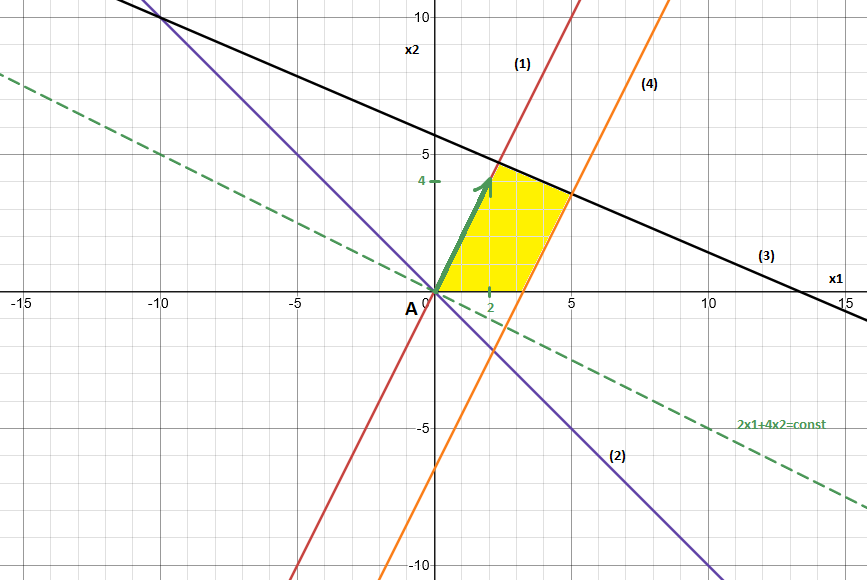
\includegraphics[width=\textwidth]{1-1.png}
\begin{center}
  Рис. 1.1 Область допустимых решений
\end{center}

Для линий уровня $2x_1+4x_2 = \text{const}$ строим нормальный вектор $\vec{n} = (2,4)$ перпендикулярно вектору нормаль построим одну из линий уровня Перемещаем её в направлении вектора $\vec{n}$ до опорной прямой. Для определения координат точки A решаем систему уравнений:\\

\begin{math}
  \begin{cases}
    2x_1-x_2 \geq 0,(1)\\
    -x_1-x_2 \leq 0,(2)\\
  \end{cases}
\end{math}\\

Получаем $x_1 = 0, x_2 = 0$ это и есть оптимальное решение. Минимальное значение целевой функции $Z(X) = 2 \cdot 0 + 4 \cdot 0 = 0$.
\newpage
\section{Транспортная задача}
Дана задача \\
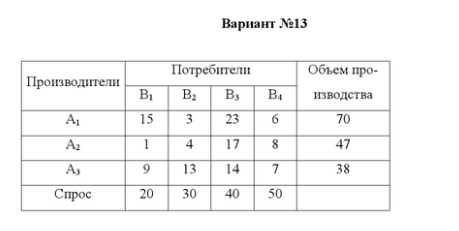
\includegraphics{2-1.png}\\

\subsection{Exel}
Создаем таблицу для ввода условий задачи и введем исходные данные:\\

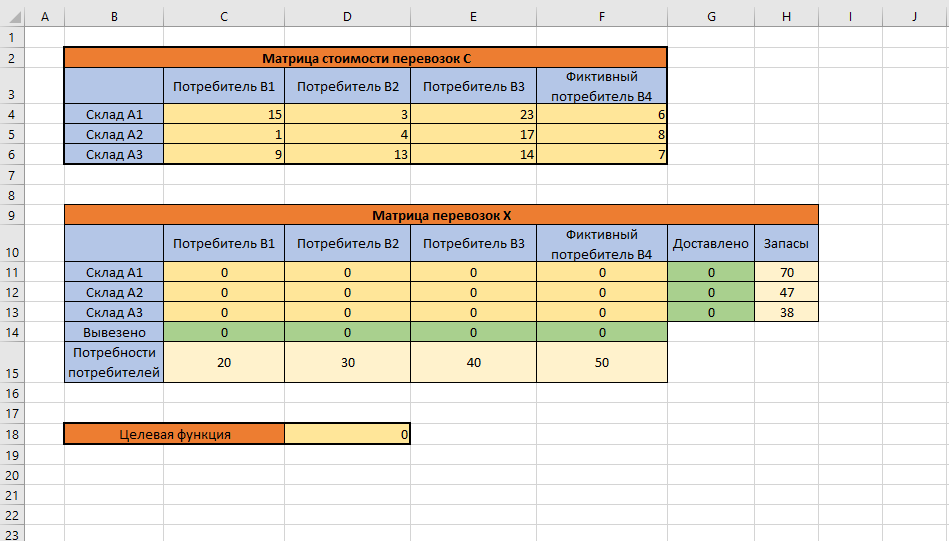
\includegraphics[width=\textwidth]{2-2.png}\\

Вводим формулы расчета для различных ячеек:
\begin{verbatim}
  D18 =SUMPRODUCT(C4:F6;C11:F13)

  G11 =SUM(C11:F11)
  G12 =SUM(C12:F12)
  G13 =SUM(C13:F13)

  C14 =SUM(C11:C13)
  D14 =SUM(D11:D13)
  E14 =SUM(E11:E13)
  F14 =SUM(F11:F13)
\end{verbatim}

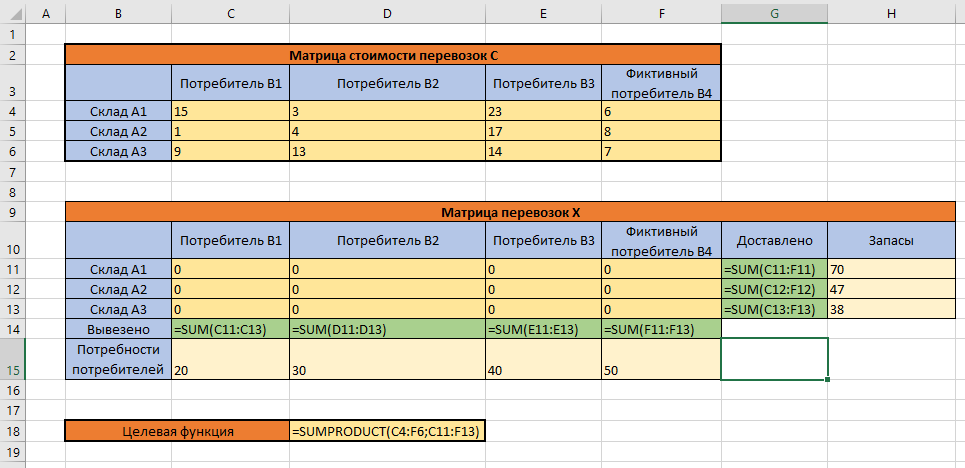
\includegraphics[width=\textwidth]{2-3.png}\\

\newpage
Заполняем окно параметров поиска решений:\\

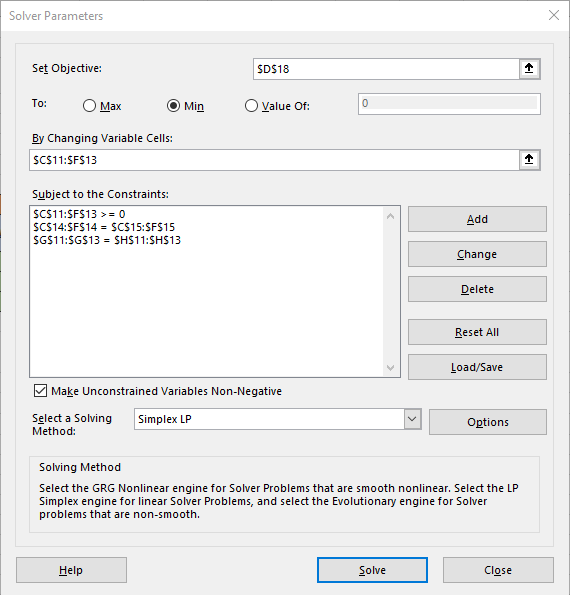
\includegraphics{2-4.png}\\

Результат: \\

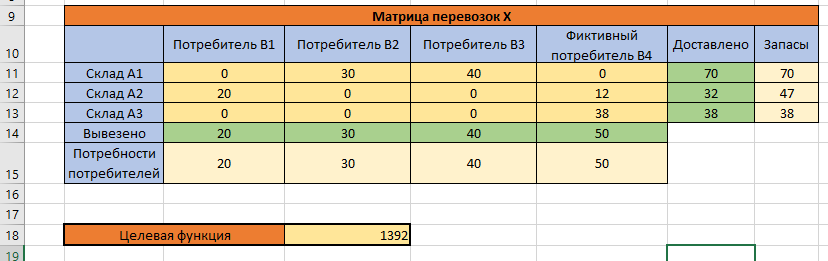
\includegraphics[width=\textwidth]{2-5.png}\\

\newpage
\subsection{Метод потенциалов(опорный план с помощью северо-западного угла)}

Задана таблица транспортной задачи:
\begin{table}[H]
\centering
\begin{tabular}{c|c|c|c|c|}
\cline{2-5}
                              & B1=20 & B2=30 & B3=40 & B4=50 \\ \hline
\multicolumn{1}{|c|}{A1 = 70} & 15    & 3     & 23    & 6     \\ \hline
\multicolumn{1}{|c|}{A2 = 47} & 1     & 4     & 17    & 8     \\ \hline
\multicolumn{1}{|c|}{A3 = 38} & 9     & 13    & 14    & 7     \\ \hline
\end{tabular}
\end{table}

Суммарные запасы груза $70+47+38=155$, а суммарное потребление $20+30+40+50=140$. Следовательно Задача является открытого типа и ее нужно закрыть вводом нового потребителя с стоимостью перевозок 0 и потребностями $155-140=15$.
\begin{table}[H]
\centering
\begin{tabular}{c|c|c|c|c|c|}
\cline{2-6}
                              & B1=20 & B2=30 & B3=40 & B4=50 & B5=15 \\ \hline
\multicolumn{1}{|c|}{A1 = 70} & 15    & 3     & 23    & 6     & 0     \\ \hline
\multicolumn{1}{|c|}{A2 = 47} & 1     & 4     & 17    & 8     & 0     \\ \hline
\multicolumn{1}{|c|}{A3 = 38} & 9     & 13    & 14    & 7     & 0     \\ \hline
\end{tabular}
\end{table}

Метод северо-западного угла:
\begin{table}[H]
\centering
\begin{tabular}{|c|c|c|c|c|c|c|}
\hline
            & B1      & B2    & B3    & B4    & B5    & Запасы \\ \hline
A1          & 15[20]  & 3[30] & 23[20]& 6[0]  & 0[0]  & 70     \\ \hline
A2          & 1[0]    & 4[0]  & 17[20]& 8[27] & 0[0]  & 47     \\ \hline
A3          & 9[0]    & 13[0] & 14[0] & 7[23] & 0[15] & 38     \\ \hline
Потребности & 20      & 30    & 40    & 50    & 15    &        \\ \hline
\end{tabular}
\end{table}

\begin{math}
  7 = m+n-1 = 3+5-1 = 7 \Rightarrow \textsc{невырожденный}\\
  F(x)=\sum_{i=1}^3\sum_{j=1}^5 c_{ij}x_{ij} = 15\cdot20+3\cdot30+23\cdot20+17\cdot20+8\cdot27+7\cdot23+0\cdot15 = 1567
\end{math}\\

Метод потенциалов:\\
1. Находим предварительные потенциалы $u_i,v_j$, по заданному плану, где $u_i+v_j=c_{ij}, u_1 = 0$\\
2. Проверяем на оптимальность, где не существуют $u_i+v_j > c_{ij}$ \\
3. Выбераем максимальную оценку свобдной клетки\\
4. Строим цикл, чередуя +/-, вершина цикла, выбранная свободная клетка начинается с '+', выбераем наименьшей объем груза из ячеек с '-', и прибавляем это значение к элементам цикла\\

\newpage
1-итерация:\\
\begin{equation*}
  1)\begin{split}
    u_1 + v_1 = 15; v_1 = 15-0 = 15\\
    u_1 + v_2 = 3; v_2 = 3-0 = 3\\
    u_1 + v_3 = 23; v_3 = 23-0 = 23\\
    u_2 + v_3 = 17; u_2 = 17-23 = -6\\
    u_2 + v_4 = 8; v_4 = 8-(-6) = 14\\
    u_3 + v_4 = 7; u_3 = 7-14 = -7\\
    u_3 + v_5 = 0; v_5 = 0-(-7) = 7\\
  \end{split}
  \qquad  
  2)\begin{split}
    \Delta_{14} = 0 + 14 - 6 = 8 > 0 \\
    \Delta_{15} = 0 + 7 - 0 = 7 > 0 \\
    \Delta_{21} = -6 + 15 - 1 = 8 > 0 \\
    \Delta_{22} = -6 + 3 - 4 = -7 < 0 \\
    \Delta_{25} = -6 + 7 - 0 = 1 > 0 \\
    \Delta_{31} = -7 + 15 - 9 = -1 < 0 \\
    \Delta_{32} = -7 + 3 - 13 = -17 < 0 \\
    \Delta_{33} = -7 + 23 - 14 = 2 > 0 \\
  \end{split}
\end{equation*}

\begin{math}
  3) \max(8,7,8,1,2)= 8 \Rightarrow \max(1_{21},6_{14}) = 6
\end{math}
\begin{table}[H]
\centering
\begin{tabular}{|c|c|c|c|c|c|c|}
\hline
            & B1(V1=15)& B2(V2=3) & B3(V3=23) & B4(V4=14) & B5(V5=7)  & Запасы \\ \hline
A1(U1=0)    & 15[20]   & 3[30]    & 23[20]-   & 6[0]+     & 0[0]      & 70     \\ \hline
A2(U2=-6)   & 1[0]     & 4[0]     & 17[20]+   & 8[27]-    & 0[0]      & 47     \\ \hline
A3(U3=-7)   & 9[0]     & 13[0]    & 14[0]     & 7[23]     & 0[15]     & 38     \\ \hline
Потребности & 20       & 30       & 40        & 50        & 15        &        \\ \hline
\end{tabular}
\end{table}

\begin{center}
  $\Downarrow$\\
  4) $(1,4)\rightarrow(1,3)\rightarrow(2,3)\rightarrow(2,4)\rightarrow(1,4)$\\
  $\min(20,27) = 20$
\end{center}
\begin{table}[H]
\centering
\begin{tabular}{|c|c|c|c|c|c|c|}
\hline
            & B1(V1=15)& B2(V2=3) & B3(V3=23) & B4(V4=14) & B5(V5=7)  & Запасы \\ \hline
A1(U1=0)    & 15[20]   & 3[30]    & 23[0]     & 6[20]     & 0[0]      & 70     \\ \hline
A2(U2=-6)   & 1[0]     & 4[0]     & 17[40]    & 8[07]     & 0[0]      & 47     \\ \hline
A3(U3=-7)   & 9[0]     & 13[0]    & 14[0]     & 7[23]     & 0[15]     & 38     \\ \hline
Потребности & 20       & 30       & 40        & 50        & 15        &        \\ \hline
\end{tabular}
\end{table}

2-итерация:\\
\begin{equation*}
  1)\begin{split}
    u_1 + v_1 = 15; v_1 = 15-0 = 15\\
    u_1 + v_2 = 3; v_2 = 3-0 = 3\\
    u_1 + v_4 = 6; v_4 = 6-0 = 6\\
    u_2 + v_4 = 8; u_2 = 8-6 = 2\\
    u_2 + v_3 = 17; v_3 = 17-2 = 15\\
    u_3 + v_4 = 7; u_3 = 7-6 = 1\\
    u_3 + v_5 = 0; v_5 = 0-1 = -1\\
  \end{split}
  \qquad  
  2)\begin{split}
    \Delta_{13} = 0 + 15 - 23 = -8 < 0 \\
    \Delta_{15} = 0 + (-1) - 0 = -1 < 0 \\
    \Delta_{21} = 2 + 15 - 1 = 16 > 0 \\
    \Delta_{22} = 2 + 3 - 4 = -1 < 0 \\
    \Delta_{25} = 2 + -1 - 0 = 1 > 0 \\
    \Delta_{31} = 1 + 15 - 9 = 7 > 0 \\
    \Delta_{32} = 1 + 3 - 13 = -9 < 0 \\
    \Delta_{33} = 1 + 15 - 14 = 2 > 0 \\
  \end{split}
\end{equation*}

\begin{math}
  3) \max(16,1,7,2)= 16 \Rightarrow \max(16_{21}) = 1
\end{math}
\begin{table}[H]
\centering
\begin{tabular}{|c|c|c|c|c|c|c|}
\hline
            & B1(V1=15)& B2(V2=3) & B3(V3=15) & B4(V4=6)  & B5(V5=-1) & Запасы \\ \hline
A1(U1=0)    & 15[20]-  & 3[30]    & 23[20]    & 6[0]+     & 0[0]      & 70     \\ \hline
A2(U2=2)    & 1[0]+    & 4[0]     & 17[40]    & 8[7]-     & 0[0]      & 47     \\ \hline
A3(U3=1 )   & 9[0]     & 13[0]    & 14[0]     & 7[23]     & 0[15]     & 38     \\ \hline
Потребности & 20       & 30       & 40        & 50        & 15        &        \\ \hline
\end{tabular}
\end{table}

\begin{center}
  $\Downarrow$\\
  4) $(2,1)\rightarrow(1,1)\rightarrow(1,4)\rightarrow(2,4)\rightarrow(2,1)$\\
  $\min(20,7) = 7$
\end{center}
\begin{table}[H]
\centering
\begin{tabular}{|c|c|c|c|c|c|c|}
\hline
     & B1       & B2       & B3)       & B4        & B5        & Запасы \\ \hline
A1   & 15[13]   & 3[30]    & 23[0]     & 6[27]     & 0[0]      & 70     \\ \hline
A2   & 1[7]     & 4[0]     & 17[40]    & 8[0]      & 0[0]      & 47     \\ \hline
A3   & 9[0]     & 13[0]    & 14[0]     & 7[23]     & 0[15]     & 38     \\ \hline
Потребности & 20       & 30       & 40        & 50        & 15        &        \\ \hline
\end{tabular}
\end{table}

3-итерация:\\
\begin{equation*}
  1)\begin{split}
    u_1 + v_1 = 15; v_1 = 15-0 = 15\\
    u_2 + v_1 = 1; u_2 = 1-15 = -14\\
    u_2 + v_3 = 17; v_3 = 17+14 = 31\\
    u_1 + v_2 = 3; v_2 = 3-0 = 3\\
    u_1 + v_4 = 6; v_4 = 6-0 = 6\\
    u_3 + v_4 = 7; u_3 = 7-6 = 1\\
    u_3 + v_5 = 0; v_5 = 0-1 = -1\\
  \end{split}
  \qquad  
  2)\begin{split}
    \Delta_{13} = 0+31-23= 8 > 0 \\
    \Delta_{31} = 1+15-9= 7 > 0 \\
    \Delta_{33} = 1+31-14= 18 > 0 \\
  \end{split}
\end{equation*}

\begin{math}
  3) \max(8,7,18)= 18 \Rightarrow \max(18_{33}) = 14
\end{math}
\begin{table}[H]
\centering
\begin{tabular}{|c|c|c|c|c|c|c|}
\hline
            & B1(V1=15)& B2(V2=3) & B3(V3=31) & B4(V4=6)  & B5(V5=-1) & Запасы \\ \hline
A1(U1=0)    & 15[13]-  & 3[30]    & 23[0]     & 6[27]+    & 0[0]      & 70     \\ \hline
A2(U2=-14)  & 1[7]+    & 4[0]     & 17[40]-   & 8[0]      & 0[0]      & 47     \\ \hline
A3(U3=1 )   & 9[0]     & 13[0]    & 14[0]+    & 7[23]-    & 0[15]     & 38     \\ \hline
Потребности & 20       & 30       & 40        & 50        & 15        &        \\ \hline
\end{tabular}
\end{table}

\begin{center}
  $\Downarrow$\\
  4) $(3,3)\rightarrow(2,3)\rightarrow(2,1)\rightarrow(1,1)\rightarrow(1,4)\rightarrow(3,4)\rightarrow(3,3)$\\
  $\min(13,23,40) = 13$
\end{center}
\begin{table}[H]
\centering
\begin{tabular}{|c|c|c|c|c|c|c|}
\hline
     & B1       & B2       & B3        & B4        & B5        & Запасы \\ \hline
A1   & 15[0]    & 3[30]    & 23[0]     & 6[40]     & 0[0]      & 70     \\ \hline
A2   & 1[20]    & 4[0]     & 17[27]    & 8[0]      & 0[0]      & 47     \\ \hline
A3   & 9[0]     & 13[0]    & 14[13]    & 7[10]     & 0[15]     & 38     \\ \hline
Потребности & 20       & 30       & 40        & 50        & 15        &        \\ \hline
\end{tabular}
\end{table}

4-итерация:\\
\begin{equation*}
  1)\begin{split}
    v_2= 3 - u_1 = 3-0 = 3\\
    v_4= 6 - u_1 = 6-0 = 6\\
    u_3= 7 - v_4 = 7-6 = 1\\
    v_3= 14 - u_3 = 14-1 = 13\\
    u_2= 17 - v_3 = 17-13 = 4\\
    v_1= 1 - u_2 = 1-4 = -3\\
    v_5= 0 - u_3 = 0-1 = -1\\
  \end{split}
  \qquad  
  2)\begin{split}
    \Delta_{22} =4+3-4=3> 0 \\
    \Delta_{24} =4+6-8=2> 0 \\
    \Delta_{25} =4-1-0=3> 0 \\
  \end{split}
\end{equation*}

\begin{math}
  3) \max(3,2,3)= 3 \Rightarrow \max(3_{22}) = 4
\end{math}
\begin{table}[H]
\centering
\begin{tabular}{|c|c|c|c|c|c|c|}
\hline
            & B1(V1=-3)& B2(V2=3) & B3(V3=13) & B4(V4=6)  & B5(V5=-1) & Запасы \\ \hline
A1(U1=0)    & 15[0]    & 3[30]-   & 23[0]     & 6[40]+    & 0[0]      & 70     \\ \hline
A2(U2=4)    & 1[20]    & 4[0]+    & 17[27]-   & 8[0]      & 0[0]      & 47     \\ \hline
A3(U3=1 )   & 9[0]     & 13[0]    & 14[13]+   & 7[10]-    & 0[15]     & 38     \\ \hline
Потребности & 20       & 30       & 40        & 50        & 15        &        \\ \hline
\end{tabular}
\end{table}

\begin{center}
  $\Downarrow$\\
  4) $(2,2)\rightarrow(1,2)\rightarrow(1,4)\rightarrow(3,4)\rightarrow(3,3)\rightarrow(2,3)\rightarrow(2,2)$\\
  $\min(30,10,27) = 10$
\end{center}
\begin{table}[H]
\centering
\begin{tabular}{|c|c|c|c|c|c|c|}
\hline
     & B1       & B2       & B3        & B4        & B5        & Запасы \\ \hline
A1   & 15[0]    & 3[20]    & 23[0]     & 6[50]     & 0[0]      & 70     \\ \hline
A2   & 1[20]    & 4[10]    & 17[17]    & 8[0]      & 0[0]      & 47     \\ \hline
A3   & 9[0]     & 13[0]    & 14[23]    & 7[0]      & 0[15]     & 38     \\ \hline
Потребности & 20       & 30       & 40        & 50        & 15        &        \\ \hline
\end{tabular}
\end{table}

5-итерация:\\
\begin{equation*}
  1)\begin{split}
    v_2= 3 - u_1 = 3-0 = 3\\
    u_2= 4 - v_2 = 4-3 = 1\\
    v_1= 1 - u_2 = 1-1 = 0\\
    v_3= 17 - u_2 = 17-1 = 16\\
    u_3= 14 - v_3 = 14-16 = -2\\
    v_5= 0 - u_3 = 0+2 = 2\\
    v_4= 6 - u_1 = 6-0 = 6\\
  \end{split}
  \qquad  
  2)\begin{split}
    \Delta_{15} =0+2-0=2> 0 \\
    \Delta_{25} =1+2-0=3> 0 \\
  \end{split}
\end{equation*}

\begin{math}
  3) \max(2,3)= 3 \Rightarrow \max(3_{25}) = 0
\end{math}
\begin{table}[H]
\centering
\begin{tabular}{|c|c|c|c|c|c|c|}
\hline
            & B1(V1=0 )& B2(V2=3) & B3(V3=16) & B4(V4=6)  & B5(V5=2 ) & Запасы \\ \hline
A1(U1=0)    & 15[0]    & 3[20]    & 23[0]     & 6[50]     & 0[0]      & 70     \\ \hline
A2(U2=1)    & 1[20]    & 4[10]    & 17[17]-   & 8[0]      & 0[0]+     & 47     \\ \hline
A3(U3=-2)   & 9[0]     & 13[0]    & 14[23]+   & 7[0]      & 0[15]-    & 38     \\ \hline
Потребности & 20       & 30       & 40        & 50        & 15        &        \\ \hline
\end{tabular}
\end{table}

\begin{center}
  $\Downarrow$\\
  4) $(2,5)\rightarrow(3,5)\rightarrow(3,3)\rightarrow(2,3)\rightarrow(2,5)$\\
  $\min(17,15) = 15$
\end{center}
\begin{table}[H]
\centering
\begin{tabular}{|c|c|c|c|c|c|c|}
\hline
     & B1       & B2       & B3        & B4        & B5        & Запасы \\ \hline
A1   & 15[0]    & 3[20]    & 23[0]     & 6[50]     & 0[0]      & 70     \\ \hline
A2   & 1[20]    & 4[10]    & 17[2]     & 8[0]      & 0[15]     & 47     \\ \hline
A3   & 9[0]     & 13[0]    & 14[38]    & 7[0]      & 0[0]      & 38     \\ \hline
Потребности & 20       & 30       & 40        & 50        & 15        &        \\ \hline
\end{tabular}
\end{table}

6-итерация:\\
\begin{equation*}
  1)\begin{split}
    v_2= 3 - u_1 = 3-0 = 3\\
    u_2= 4 - v_2 = 4-3 = 1\\
    v_1= 1 - u_2 = 1-1 = 0\\
    v_3= 17 - u_2 = 17-1 = 16\\
    u_3= 14 - v_3 = 14-16 = -2\\
    v_5= 0 - u_2 = 0-1 = -1\\
    v_4= 6 - u_1 = 6-0 = 6\\
  \end{split}
  \qquad  
  2)\begin{split}
    \Delta_{11} = 0+0-15 \leq 0 \\
    \Delta_{13} = 0+16-23 = -7 \leq 0 \\
    \Delta_{15} = 0-1-0 = -1 \leq 0 \\
    \Delta_{24} = 1+6-8 = -1 \leq 0 \\
    \Delta_{31} = -2+0-0 = -11 \leq 0 \\
    \Delta_{32} = -2+3-13 = -12 \leq 0 \\
    \Delta_{34} = -2+6-7 = -3 \leq 0 \\
    \Delta_{35} = -2-1-0 = -3 \leq 0 \\
  \end{split}
\end{equation*}

\begin{table}[H]
\centering
\begin{tabular}{|c|c|c|c|c|c|c|}
\hline
     & B1       & B2       & B3        & B4        & B5        & Запасы \\ \hline
A1   & 15[0]    & 3[20]    & 23[0]     & 6[50]     & 0[0]      & 70     \\ \hline
A2   & 1[20]    & 4[10]    & 17[2]     & 8[0]      & 0[15]     & 47     \\ \hline
A3   & 9[0]     & 13[0]    & 14[38]    & 7[0]      & 0[0]      & 38     \\ \hline
Потребности & 20       & 30       & 40        & 50        & 15        &        \\ \hline
\end{tabular}
\end{table}

Опорный план является оптимальным, т.к. все оценки свободных клеток удовлетворяют условию $u_i+v_j\leq c_{ij}$. Затраты: $F(x)=3\cdot20+6\cdot50+1\cdot20+4\cdot10+17\cdot2+0\cdot15+14\cdot38 = 986$

% 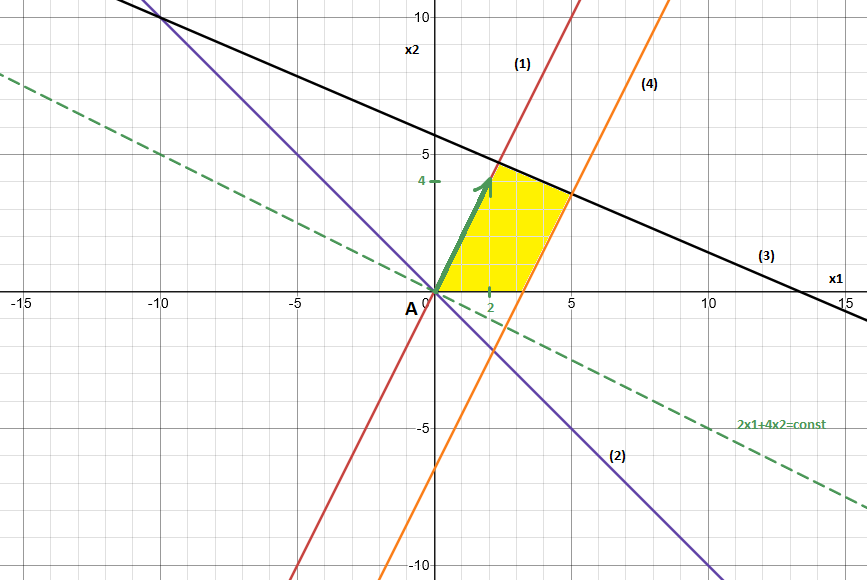
\includegraphics[width=\textwidth]{1-1.png}\\

\end{document}